\documentclass[a4paper,10pt]{article}
\usepackage[utf8]{inputenc}
\usepackage{graphicx}
\usepackage{amsmath}
\usepackage{amssymb}
\usepackage{amsthm}
\usepackage{booktabs}
\usepackage{caption}
\usepackage{geometry}
%\usepackage{hyperref}
\usepackage{makeidx}
\usepackage{microtype}
\usepackage{subfig}
\usepackage{tabularx}
\usepackage{url}
\usepackage{varioref}
\usepackage[italian]{babel}
\usepackage{xcolor}
\usepackage{multicol}
\usepackage{mathtools}
\usepackage{booktabs}
\usepackage{gensymb}


\title{Laboratorio I: Misura dell'indice di rifrazione\\Acqua e plexiglass\\
\begin{large}
Dipartimento di Fisica E.Fermi - Università di Pisa
\end{large}}

\author{Di Ubaldo Gabriele \\Torosantucci Andrea \\ Giannelli Martina}
\date{9 Marzo 2016}

\begin{document}

\maketitle

\tableofcontents

%%%%%%%%%%%%%%%%%%%%%%%%%%%%%%%%%%%%%%%%%%%%%%%%%%%%%%%%%%%%%%%%%%%%%%%%%%%%%%%%%%%%%%%%%%%%%%%%%%%%%%%%%%%%%%%%%%%%%%%%%%%%%%%%%%%%%%%%%%%%%%%%%%%%%%%%%%%%%%%%%%%%%%%%%%%%%%%%%%%
\section{Introduzione}
\subsection{Teoria}
\textbf{Obiettivo:} Misurare gli indici di rifrazione dell'acqua e del plexiglass.\\
\textbf{Plexiglass:} La legge di Snell descrive l'angolo di rifrazione prodotto quando un raggio di luce passa da un mezzo con indice $n_1$ ad un altro mezzo con indice $n_2$.
\begin{equation}
 n_1 \sin\theta_i=n_2\sin\theta_r
\end{equation}
Consideriamo l'indice di rifrazione dell'aria $n_1=1$ come per il vuoto.
\\ \textbf{Acqua:}L'ottica geometrica descrive la trasformazione di un raggio di luce passante per un diottro e due mezzi diversi:
\begin{equation}
 \frac{n_2}{p}+\frac{n_1}{q}=\frac{(n_2-n_1)}{r}
\end{equation}
che è una relazione lineare tra $\frac{1}{q}$ e $\frac{1}{p}$

\subsection{Apparato sperimentale}
\begin{itemize}
\item{Banco ottico con sorgente luminosa}
\item{Semicilindro di plexiglass}
\item{Diottro sferico riempito d'acqua}
\item{Metro a nastro con risoluzione di $1mm$}
\end{itemize}

%%%%%%%%%%%%%%%%%%%%%%%%%%%%%%%%%%%%%%%%%%%%%%%%%%%%%%%%%%%%%%%%%%%%%%%%%%%%%%%%%%%%%%%%%%%%%%%%%%%%%%%%%%%%%%%%%%%%%%%%%%%%%%%%%%%%%%%%%%%%%%%%%%%%%%%%%%%%%%%%%%%%%%%%%%%%%%%%%%%
\section{Esperimento}
\subsection{Acquisizione misure}
\textbf{Plexiglass:} Posizioniamo il semicilindro di plexiglass sulla sua sagoma nella carta millimetrata e collimiamo il raggio di luce muovendo ad una distanza ottimale la fessura davanti alla sorgente di di luce. Abbiamo girato il semicilindro per variare l'angolo di incidenza mantenendo costante il punto di incidenza nel centro.
La nostra stima dell'errore commesso è di $0.5 u.a.$
Abbiamo preso 10 misure di angoli di incidenza e rifrazione.
\\ 
\textbf{Acqua:}Poniamo la sorgente ad una distanza arbitraria dal diottro cercando di esplorare il massimo ventaglio di misure possibili e  muoviamo lo schermo finchè l'immagine non è a fuoco.
A quel punto misuriamo $p$ e $q$.
La nostra stima dell'errore commesso è di $1cm$

\subsection{Analisi Dati}
\textbf{Plexiglas}

I dati misurati per il plexiglas sono i seguenti:

\begin{table}[!htb]
\centering
\caption{Plexiglas}
\label{my-labl}
\begin{tabular}{l|llllllllll}
$\sin\theta_r(u.a.)$ & 3.5 & 4.5 & 9.5 & 11.5 & 13.5 & 16.5 & 20.5 & 21.5& 26.5 & 27.5 \\ \hline
$\sin\theta_i(u.a.)$ & 5.5 & 6.5 & 12.5 & 16.5 & 19.5 & 23.5 & 30.5 & 31.5& 39.5 & 40.5
\end{tabular}
\end{table}
\pagebreak

 \begin {figure}[!htb]
\begin{center}
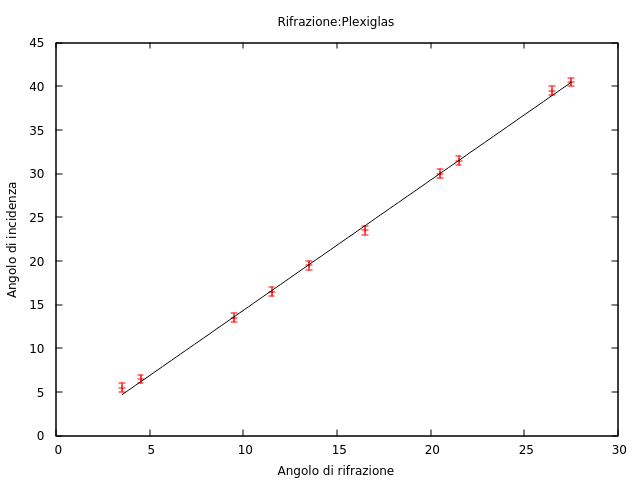
\includegraphics[width=10cm]{/home/zerch/Documents/UNIPI/LAB1/10Rifrazione/dati/graf-plexi.png}
\end{center}
\end{figure}

Il fit lineare ci fornisce una stima dell'indice di rifrazione del plexiglas $n=1.49\pm0.023$ che è compatibile con il valore noto di $1.48$. Per il fit si ha $\chi2=10.64$ e $\chi2_r=1.33$.

\textbf{Acqua}

I dati misurati per il diottro sono i seguenti:

\begin{table}[!htb]
\centering
\caption{Misure Diottro}
\label{my-labl}
\begin{tabular}{l|llllll}
$p$ & 48.5 & 43.5 & 41.5 & 38.5 & 34.5 & 33.5 \\ \hline
$q$ & 43.5 & 47.5 & 54.5 & 63.5 & 82.5 & 86.5
\end{tabular}
\end{table}
\pagebreak
 \begin {figure}[!htb]
\begin{center}
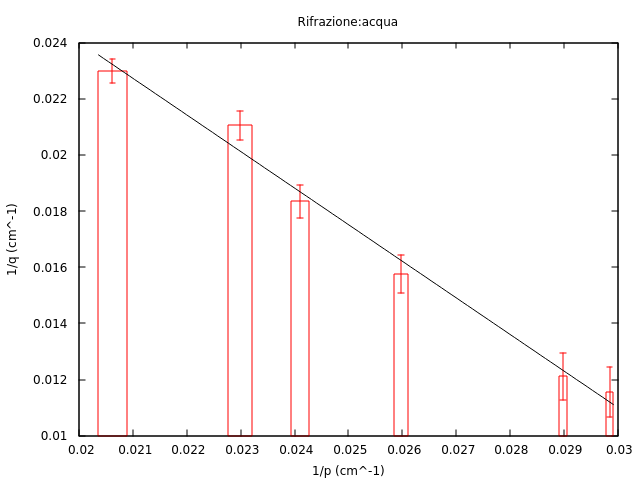
\includegraphics[width=10cm]{/home/zerch/Documents/UNIPI/LAB1/10Rifrazione/dati/graf-acqua.png}
\end{center}
\end{figure}

Il fit lineare ci forrnisce una stima dell'indice di rifrazione dell'acqua $n= 1.30 \pm 0.08$ che è compatibile con il valore noto $1.32$ Per il fit si ha $\chi2=4.44$ e $\chi2_r=1.11$

\section{Conclusione}
I risultati dimostrano la validità del modello fisico utilizzato come si vede dal calcolo del $\chi2$ per entrambi i fit. Le misure degli indici di rifrazione sono entrambe compatibili entro l'errore con il valore noto.
\end{document}


